\documentclass{article}
\usepackage{fullpage}
\usepackage{graphicx}
\usepackage{amsmath}

\title{Shor}
\author{Jacques Carette \and Gerardo Ortiz \and Amr Sabry}

\begin{document}
\maketitle

\newcommand{\st}[5]{\ensuremath{| #1, #2, #3, #4, #5 \rangle}}
\newcommand{\ket}[1]{\ensuremath{| #1 \rangle}}

%%%%%%%%%%%%%%%%%%%%%%%%%%%%%%%%%%%%%%%%%%%%%%%%%%%%%%%%%%%%%%%%%%%%%%%%%%%%%%%%%%
\section{Claims}

\paragraph*{Claim I.}
An efficient generate-and-test algorithm of expmod would allow an
efficient classical implementation of Shor's algorithm.

\paragraph*{Claim II.}
It is possible to realize an efficient generate-and-test algorithm for
expmod by using partial evaluation and reverse execution.

%%%%%%%%%%%%%%%%%%%%%%%%%%%%%%%%%%%%%%%%%%%%%%%%%%%%%%%%%%%%%%%%%%%%%%%%%%%%%%%%%%
\section{Purity Analysis of Shor's Algorithm}

No entanglement; conjecture that it is implementable using classical waves. 

%%%%%%%%%%%%%%%%%%%%%%%%%%%%%%%%%%%%%%%%%%%%%%%%%%%%%%%%%%%%%%%%%%%%%%%%%%%%%%%%%%
\section{Generate-and-Test Shor}

Here is a way of writing a classical algorithm that mimics the
structure of Shor's algorithm:

\begin{verbatim}
generateAndTest :: (Integer -> Integer) -> Integer -> Integer -> [Integer]
generateAndTest f range obs =
  map fst [ (x, f x) | x <- [0..range], f x == obs]

shor :: Integer -> IO (Integer,Integer)
shor n = 
  do x <- randomRIO (2, n - 1)
     let f r = powModInteger x r n                       
     test <- randomRIO (0, (n * n))
     let (a : b : _) = generateAndTest f (n * n) (f test)
     let period = b - a                                  
     let p1 = x ^ (period `div` 2) - 1                   
     let p2 = x ^ (period `div` 2) + 1                   
     return (gcd n p1, gcd n p2)                         
\end{verbatim}

All computations in \verb|shor| are trivial except the call to
\verb|generateAndTest|. If we had an efficient way of implementing
this functionality we would have an efficient factoring algorithm.     

%%%%%%%%%%%%%%%%%%%%%%%%%%%%%%%%%%%%%%%%%%%%%%%%%%%%%%%%%%%%%%%%%%%%%%%%%%%%%%%%%%
\section{Example I: Adder}

We illustrate the idea of partial reverse evaluation using a small example.

\begin{center}
  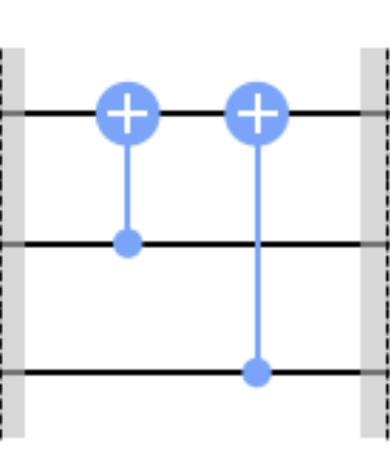
\includegraphics[scale=0.5]{bac-adder.png}
\end{center}

Say we fix the input for the top wire to be 0 and the output to be
1. We can reason as follows:

\begin{itemize}
\item Start backwards evaluation with the state \ket{1,x,y}.
\item If $y=0$, the top wire remains 1; and if $y=1$ the top wire is
  negated to 0. In otherwise, the top wire has the value
  $\overline{y}$ where the overline is boolean negation. The state is
  now \ket{\overline{y},x,y}.
\item If $x=0$, the top wire remains as $\overline{y}$ and if $x=1$
  the top wire becomes $y$. A little of algebra shows that the top
  wire will have the value $\overline{x \oplus y}$ where $\oplus$ is
  xor. The final state is \ket{\overline{x \oplus y}, x, y}.
\item If the boundary condition fixes the top input to be 0, then we
  want $\overline{x \oplus y}$ to be 0 which happens when $x \neq y$.  
\end{itemize}
So we propagated some information from the output to gain some
information about the input and did this efficiently.

%%%%%%%%%%%%%%%%%%%%%%%%%%%%%%%%%%%%%%%%%%%%%%%%%%%%%%%%%%%%%%%%%%%%%%%%%%%%%%%%%%
\section{Example II: IBM Shor 21}

The following figure is from the IBM experiment factoring 21.

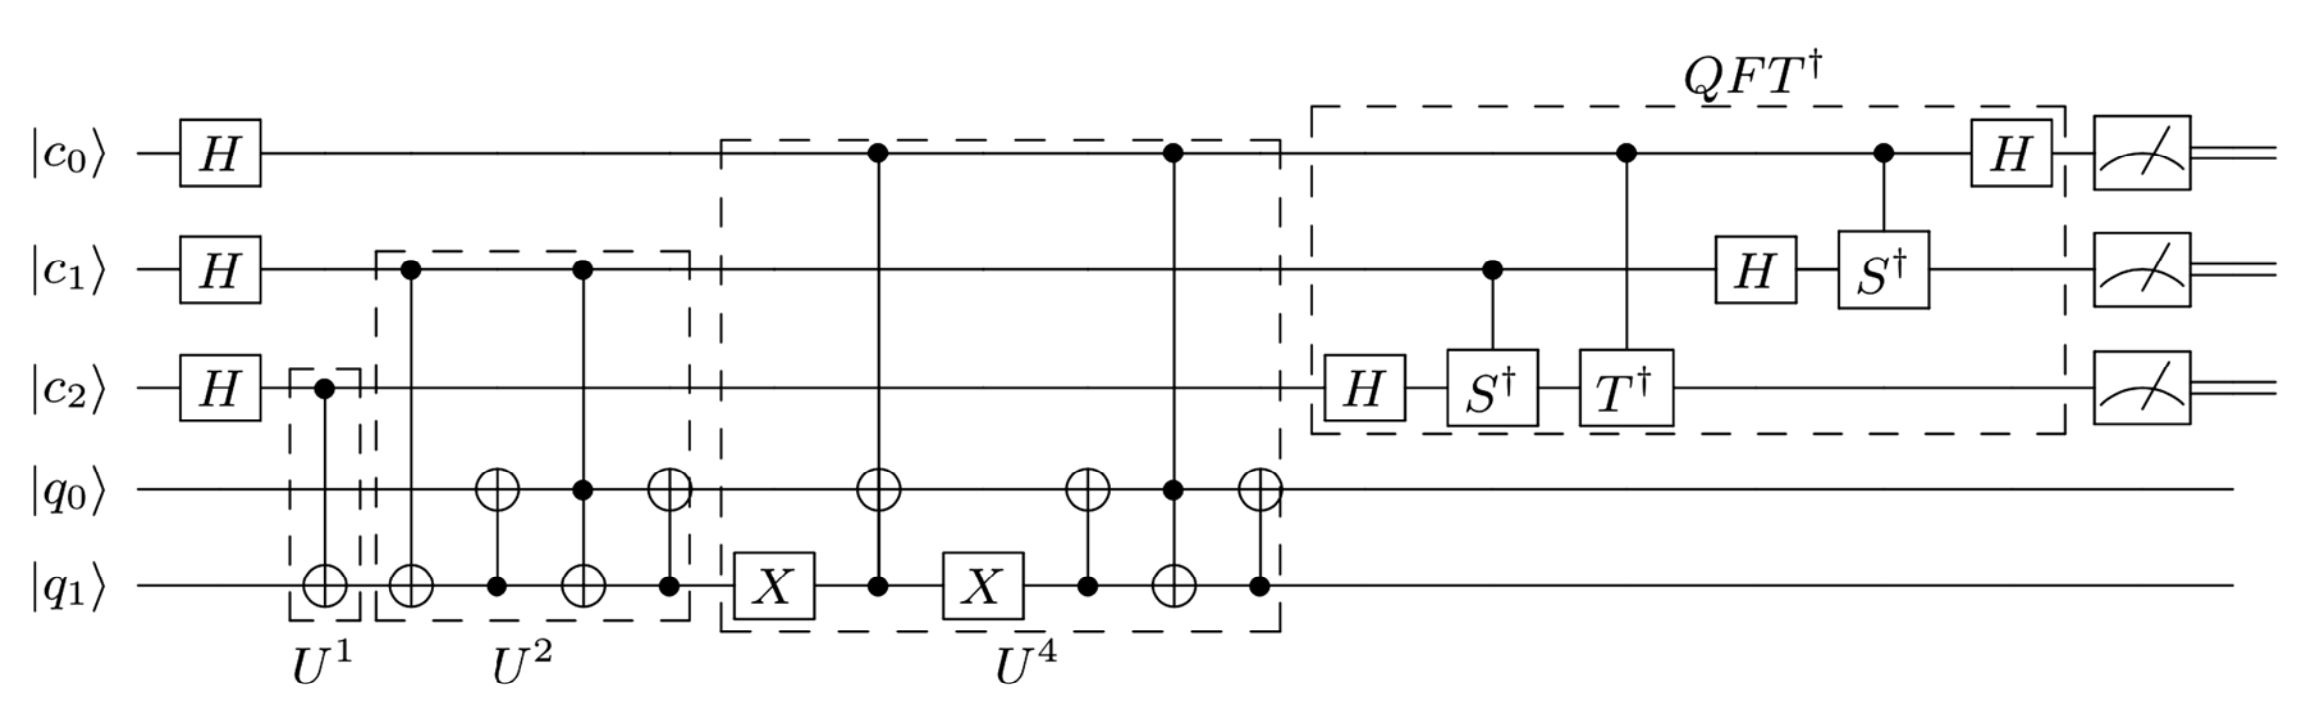
\includegraphics[scale=0.4]{ibmcircuit.png}

Ignore the Hadamard gates at the beginning and the QFT circuit at the
end. Let's start evaluating backwards starting from the partially
known state \st{a}{b}{c}{0}{1}

\begin{itemize}
\item After the first \textsf{cnot} gate (from the end), the states
  becomes \st{a}{b}{c}{1}{1}.
\item Next we have a Toffoli gate with one control wire known to be 1
  and the other is the unknown value~$a$. The resulting state
  is \st{a}{b}{c}{1}{\overline{a}} where the overline is boolean negation.
\item Next we have a \textsf{cnot} gate with the control wire
  $\overline{a}$. The result state is \st{a}{b}{c}{a}{\overline{a}}.
\item Then we have an \textsf{X} gate. The resulting state is
  \st{a}{b}{c}{a}{a}.
\item Then we have another \textsf{Toffoli} gate. The resulting state is
   \st{a}{b}{c}{0}{a}.
\item Then we have an \textsf{X} gate. The resulting state is
  \st{a}{b}{c}{0}{\overline{a}}.
\item Then we have a \textsf{cnot} gate. The result state is
    \st{a}{b}{c}{\overline{a}}{\overline{a}}.
\item Then we have a \textsf{Toffoli} gate. The resulting state is
   \st{a}{b}{c}{\overline{a}}{\overline{a}\overline{b}}.
\item Then we have a \textsf{cnot} gate. The result state is
      \st{a}{b}{c}{\overline{a}b}{\overline{a}\overline{b}}.
\item Then we have another \textsf{cnot} gate. The result state is
      \st{a}{b}{c}{\overline{a}b}{b+\overline{a}}.
\item After the last \textsf{cnot}, the final state is
      \st{a}{b}{c}{\overline{a}b}{\textsf{cx}(c,b+\overline{a})}.
\end{itemize}

Now if the initial state was supposed to be \st{a}{b}{c}{1}{1}, then we
can reason that all of $a$, $b$, and $c$ must be 0.

%%%%%%%%%%%%%%%%%%%%%%%%%%%%%%%%%%%%%%%%%%%%%%%%%%%%%%%%%%%%%%%%%%%%%%%%%%%%%%%%%%
\section{Example III: Applying the Idea to Shor (Outline)}

We want to factor 15:
\begin{itemize}
\item $N = 15$, $N^2 = 225$, so the number of qubits in the first
  register $q=8$; and the second register needs $n=4$ qubits;
\item Choose $a=8$; then $f(x) = 8^x \mod{15}$
\item The main body of the algorithm needs an efficient circuit implementing:
  \[
  U_f : \ket{x}_8\ket{0}_4 \rightarrow \ket{x}_8\ket{f(x)}_4
  \]
\item Choose a random input, say 1, compute $f(1) = 8$ and use that
  value 8 as the starting point for backwards evaluation. In other
  words, we want to run this circuit with the following partially
  known state backwards:
  \[
  \ket{x}_8\ket{8}_4
  \]
  We will match the result with $\ket{x}_8\ket{0}_4$ to derive
  constraints on $x$. We expect to see the following
  $\ket{\_,\_,\_,\_,\_,\_,0,1}$ indicating that all the values $x$ that match
  this output differ by 4.
\end{itemize}

%% *Shor> shor 15
%% 	x = 8
%% 	test = 5; obs = 8
%% 	a = 1, b = 5, period = 4
%% (3,5)

%%%%%%%%%%%%%%%%%%%%%%%%%%%%%%%%%%%%%%%%%%%%%%%%%%%%%%%%%%%%%%%%%%%%%%%%%%%%%%%%%%
\section{Partial Evaluation}

It is critical to write programs at an abstraction level that has a
rich equational theory of fine grained transformations. If
multiplication is a primitive operation then we need domain knowledge
to develop such fine grained transformations; if it expressed in
binary it is too low level. We use numbers $\mod{N}$ as our
representation and write addition, multiplication, and exponentiation
from scratch.

%% https://en.wikipedia.org/wiki/Tonelli–Shanks_algorithm

Instead of starting with exponentiation directly, we start with the
following problem that is equivalent to integer factorization. Given
$n$, $n$, and some $r$ such that $r^2 \equiv n (\mod{N})$ find
$r$. For general $N$ this is equivalent to integer
factorization. Might be an easier function to write and partial
evaluate.

Ex. \verb|f(x,y) = x * (y+1)|; I know y=1. I can conclude the output is even!


%%%%%%%%%%%%%%%%%%%%%%%%%%%%%%%%%%%%%%%%%%%%%%%%%%%%%%%%%%%%%%%%%%%%%%%%%%%%%%%%%%
\end{document}
